\documentclass[final]{beamer}
\colorlet{structure}{green!50!black}

\mode<article> % only for the article version
{
  \usepackage{fullpage}
  \usepackage{hyperref}
}
\mode<presentation>
{
%	\setbeamertemplate{background canvas}[vertical shading][bottom=red!10,top=blue!10]
%	\useinnertheme[shadow=true]{rounded}
%	\useoutertheme{shadow}
%	\usecolortheme{whale}
	\usetheme{Berkeley}
	\setbeamerfont{block title}{size={}}
%	\setbeamercovered{transparent}
%    \usefonttheme[onlysmall]{structurebold}
}

\setbeamersize{mini frame size=8cm}

\usepackage[english]{varioref}

%\usetheme{Hannover}
%\usecolortheme{dove}
%\setbeamercolor{math text}{fg=green!50!black}
%\setbeamercolor{normal text in math text}{parent=math text}

%\usepackage{pgf,pgfarrows,pgfnodes,pgfautomata,pgfheaps,pgfshade}
\usepackage{amsmath,amssymb}
%\usepackage[latin1]{inputenc}
\usepackage[utf8]{inputenc}
\usepackage{colortbl}
\usepackage[english,german,ngerman]{babel}
% Line spacing
\usepackage{setspace}
\usepackage{listings}
\lstloadlanguages{[gnu]make}
\lstset{%
 language=[gnu]make,%
 showtabs=true,%
 numbers=left,%
 stepnumber=2,%
 basicstyle=\footnotesize,%
 frameround=fttt,%
 frame=trBL}
%\usepackage{lmodern}
%\usepackage[T1]{fontenc}
\usepackage{times}
\usepackage{eurosym}
%\setbeamercovered{dynamic}


\newenvironment{ccodelisting}
{\begin{list}{}{\setlength{\leftmargin}{1em}}\item\scriptsize\bfseries}
{\end{list}}


\author{Daniel Otte \\ (daniel.otte@rub.de)}
\title{GNU-Make}
\institute{ %
\includegraphics[scale=0.1]{Labor.pdf}}
 \begin{minipage}[b]{.3\linewidth}
 
\includegraphics[scale=0.1]{Labor}
 \end{minipage}
 \hspace{0.3\linewidth}
 \begin{minipage}[b]{.3\linewidth}
 \includegraphics[scale=0.4]{Make}
 \end{minipage}
}
\date{Labor Projekttage \\ 13.-16. November 2008}

\begin{document}

%-------------------------------------------------------------------------------

\frame{\titlepage}

\section<presentation>*{}

%\begin{frame}
%  \frametitle{}
%  \tableofcontents[part=1,pausesection,hideallsubsections]
%\end{frame}

\part<presentation>{Intro}
\section{Abhängigkeiten}
\begin{frame}
	\frametitle{Beispiel Programm}
	Ein einfaches Programm aus 3 Modulen
    \begin{itemize}
      \item<2->[] 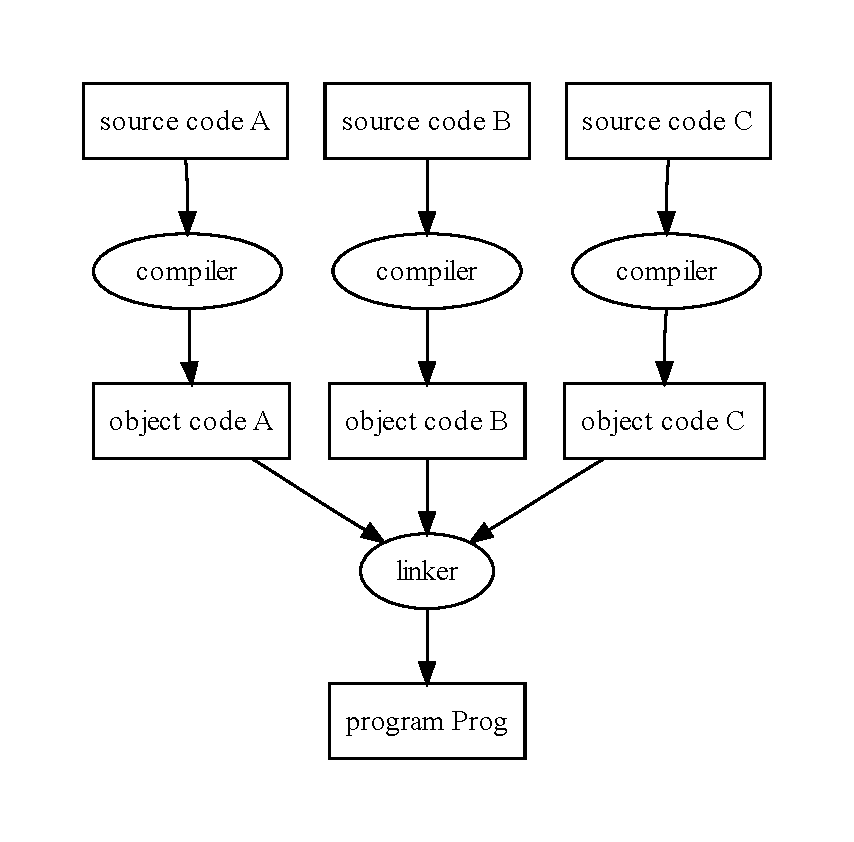
\includegraphics[scale=0.5]{prog1.pdf}      
    \end{itemize}

\end{frame}

\begin{frame}
	\frametitle{Beispiel Programm2}
	Ein anderes einfaches Programm aus 3 Modulen, mit mehr Abhängigkeiten
    \begin{itemize}
      \item<2->[] 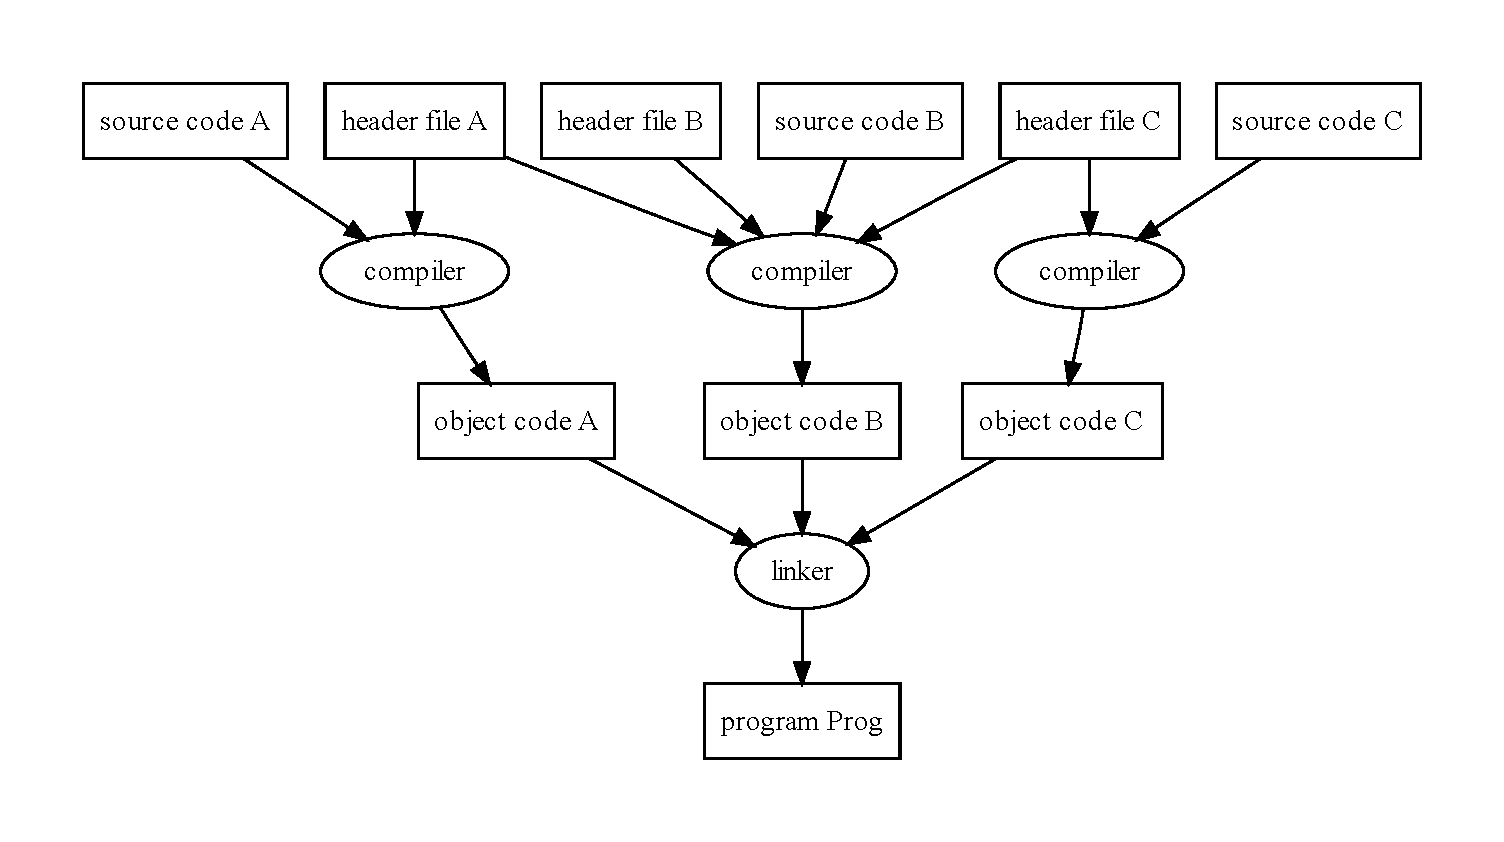
\includegraphics[scale=0.41]{prog2.pdf}      
    \end{itemize}
\end{frame}

\begin{frame}
	\frametitle{Abhängigkeiten Programm2}
	Abhängigkeiten in Programm2
    \begin{itemize}
      \item<2->[] 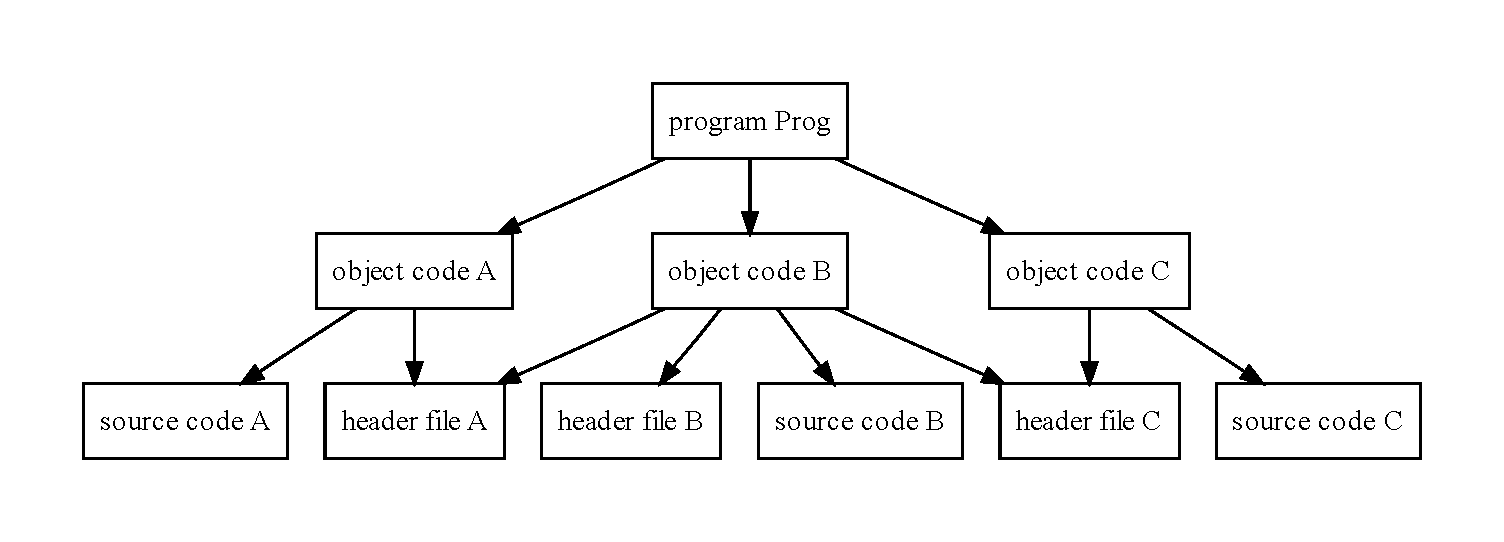
\includegraphics[scale=0.41]{prog2-dep.pdf}      
    \end{itemize}
\end{frame}


\begin{frame}
	\frametitle{Abhängigkeiten Programm2}
	Folgen einer Änderung in \textit{header file A}
    \begin{itemize}
      \item<2->[] 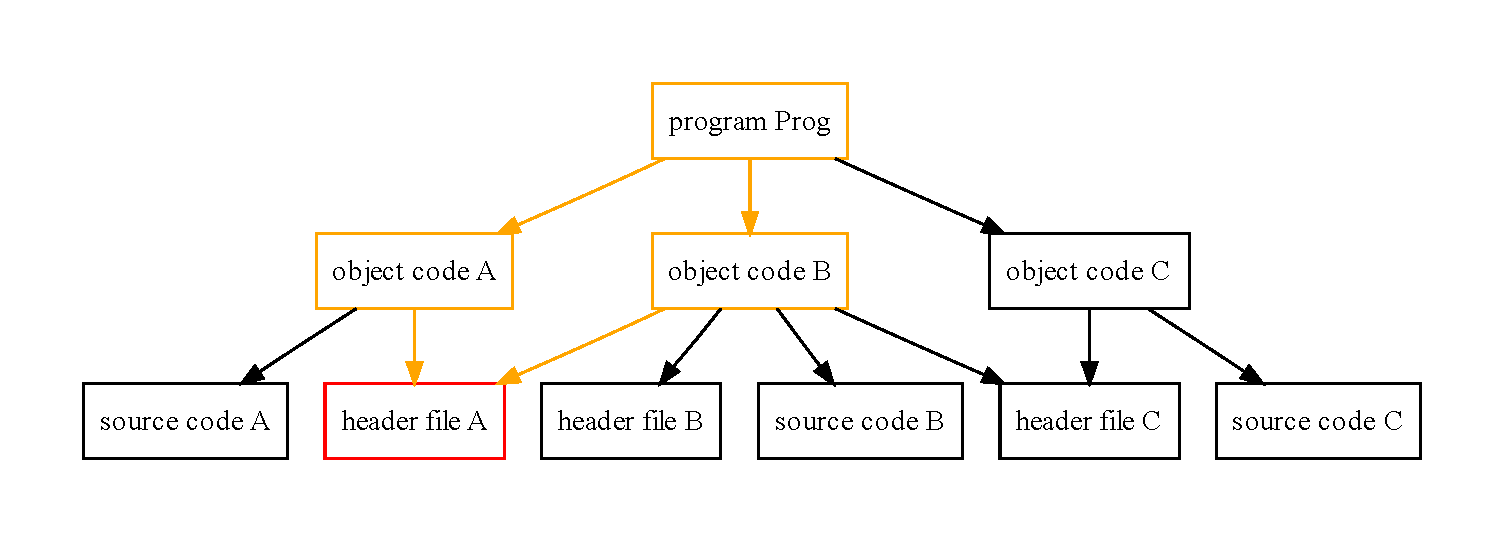
\includegraphics[scale=0.41]{prog2-dep-hl.pdf}      
    \end{itemize}
\end{frame}

\begin{frame}
	\frametitle{Was Make für dich tut}
    \begin{itemize}
      \item<2-> \large{Prüfung des Dateialters (mit Hilfe des Timestamps des Dateisystems)}
      \item<3-> \large{(neu) Erzeugen der Dateien, deren Abhängigkeiten sich geändert haben}       
    \end{itemize}
\end{frame}

\begin{frame}
	\frametitle{Was du tun must}
    \begin{itemize}
      \item<2-> \large{Make die Abhängigkeitsverhältnisse mitteilen (welche Datei hängt von wecher ab)}
      \item<3-> \large{Make mitteilen wie die Dateien zu bauen sind} 
    \end{itemize}
\end{frame} %done
\section{Make}
\begin{frame}
	\frametitle{Aufruf}
    \begin{itemize}
      \item<2->[] \texttt{make [..opts..] [target] \{target\}} 
    \end{itemize}
    Normalerweise wird dem Make-Aufruf die Liste der Ziele (targets) übergeben, dabei kann es sich handeln um:
    \begin{itemize}
      \item<3-> \underline{Dateien} die zu erstellen sind, oder
      \item<4-> spezielle \underline{Targets} die Instruktionen enthalten (Bsp. \textit{clean})
    \end{itemize}
    Wenn kein Target angegeben wird ist der Default \textit{all}.
    Die Dokumentation der Optionen findest du in der Manpage.
\end{frame}

\begin{frame}
	\frametitle{Beispiel 1}
    Ein einfaches Beispiel:
 %   \begin{block}
      \lstinputlisting{example1.make}
 %   \end{block}
\end{frame}

\begin{frame}
	\frametitle{Beispiel 2}
    Ein einfaches Beispiel mit automatischen Variablen:
 %   \begin{block}
      \lstinputlisting{example2.make}
 %   \end{block}
\begin{tabular}{|c|l|}
\hline
 Variable & Wert \\ \hline \hline
 \$@ & target \\ \hline 
 \$\^ & Abhängigkeiten \\ \hline
 \$$<$ & erste Abhängigkeit \\ \hline

\end{tabular}
\end{frame}

\begin{frame}
	\frametitle{Beispiel 3}
    Ein einfaches Beispiel mit generischen Regeln:
 %   \begin{block}
      \lstinputlisting{example3.make}
 %   \end{block}
\end{frame}      
\section{Variablen}
\begin{frame}
	\frametitle{Beispiel 4}
    Ein einfaches Beispiel mit Variablen:
 %   \begin{block}
      \lstinputlisting{example4.make}
 %   \end{block}
 
  \begin{tabular}{|c|l|}
    \hline
    \textit{variable} = \textit{wert} & Zuweisung \\ \hline 
    \$(\textit{variable}) & Referenzierung \\ \hline
  \end{tabular}
\end{frame}

%\begin{frame}
%	\frametitle{Variablen definieren, anders}
%    \begin{lstlisting}
%define varname
%   ... text ...
%endef
%    \end{lstlisting}
%\end{frame}

\begin{frame}
	\frametitle{It's all about ...}
	\begin{itemize}
    \item<2-> \huge{Strings}
    \item<3-> \huge{Lists (of Strings)}
    \end{itemize}
\end{frame}

\begin{frame}
	\frametitle{Listen sind ...}
    \begin{Large}
	Listen sind:
    \begin{itemize}
    \item<2-> Strings, die Elemente sind durch Whitespace getrennt
    \end{itemize}
    \end{Large}
\end{frame}

%\begin{frame}
%	\frametitle{Listen sind ...}
%	Listen sind:
%    \item<2-> Strings, die Elemente sind durch Whitespace getrennt
%    \end{itemize}
%\end{frame}
      
\section{Funktionen}

% $(subst from,to,text )
% $(patsubst pattern,replacement,text )
% $(strip string )
% $(findstring find,in )
% $(filter pattern ...,text )
% $(filter-out pattern ...,text )
% $(sort list )
% $(word n,text )
% $(wordlist s,e,text )
% $(words text )
% $(firstword names ...)
% $(lastword names ...)

\begin{frame}
	\frametitle{subst}
	\begin{Large}\$(subst from,to,text)\end{Large}

    \bigskip
    Führt Stringersetzung durch.
 
    \bigskip 
    Beispiel: \\
	\$(subst, ee,EE,speed tree) $\longrightarrow$ 'spEEd trEE'
\end{frame}

\begin{frame}
	\frametitle{patsubst}
	\begin{Large}\$(patsubst pattern,replacement,text)\end{Large}

	\bigskip
    Führt Musterersetzung durch.

    \bigskip 
    Beispiel: \\
	\$(patsubst, \%.c,\%.d,code.c code.h edit.c) $\longrightarrow$ 'code.d code.h edit.d'
\end{frame}

\begin{frame}
	\frametitle{strip}
	\begin{Large}\$(strip string )\end{Large}

    \bigskip
	Entfernt Whitespace am Anfang und am Ende

    \bigskip 
    Beispiel: \\
	\$(strip,   code.c code.h edit.c  ) $\longrightarrow$ 'code.d code.h edit.d'
\end{frame}

\begin{frame}
	\frametitle{findstring}
	\begin{Large}\$(findstring find,in )\end{Large}

    \bigskip
	Sucht nach \textit{find} in \textit{in} und evaluiert zu \textit{find} wenn gefunden sonst zu ' ' (empty).

    \bigskip 
    Beispiel: \\
	\$(findsring, a, a b c) $\longrightarrow$ 'a'
\end{frame}

\begin{frame}
	\frametitle{filter}
	\begin{Large}\$(filter pattern ...,text )\end{Large}

    \bigskip
	Evaluiert zu einer Liste von Strings aus \textit{text} die alle auf eins 
   (oder mehere) der \textit{pattern} passen.

    \bigskip 
    Beispiel: \\
	\$(filter, \%.c \%.s, a.c b.h c.s) $\longrightarrow$ 'a.c c.s'
\end{frame}

\begin{frame}
	\frametitle{filter-out}
	\begin{Large}\$(filter-out pattern ...,text )\end{Large}

    \bigskip
	Evaluiert zu einer Liste von Strings aus \textit{text} die alle auf keins 
    der \textit{pattern} passen.

    \bigskip 
    Beispiel: \\
	\$(filter-out, \%.c \%.s, a.c b.h c.s) $\longrightarrow$ 'b.h'
\end{frame}

\begin{frame}
	\frametitle{sort}
	\begin{Large}\$(sort list )\end{Large}

    \bigskip
	Sortiert die Liste und entfernt doppelte Einträge.

    \bigskip 
    Beispiel: \\
	\$(sort, foo bar foo lose) $\longrightarrow$ 'bar foo lose'
\end{frame}

\begin{frame}
	\frametitle{word}
	\begin{Large}\$(word n, text )\end{Large}

    \bigskip
	Evaluiert zu dem n-ten String aus Text (Indizierung beginnend bei 1).

    \bigskip 
    Beispiel: \\
	\$(word 2, foo bar foo lose) $\longrightarrow$ 'bar'
\end{frame}

\begin{frame}
	\frametitle{words}
	\begin{Large}\$(words text )\end{Large}

    \bigskip
	Evaluiert zu der Anzahl von Strings in \textit{text}.

    \bigskip 
    Beispiel: \\
	\$(words foo bar foo lose) $\longrightarrow$ '4'
\end{frame}

\begin{frame}
	\frametitle{firstword}
	\begin{Large}\$(firstwordword names ... )\end{Large}

    \bigskip
	Evaluiert zu dem ersten String in \textit{names}.

    \bigskip 
    Beispiel: \\
	\$(firstword foo bar foo lose) $\longrightarrow$ 'foo'
\end{frame}

\begin{frame}
	\frametitle{lastword}
	\begin{Large}\$(lastwordword names ... )\end{Large}

    \bigskip
	Evaluiert zu dem letzten String in \textit{names}.

    \bigskip 
    Beispiel: \\
	\$(lastword foo bar foo lose) $\longrightarrow$ 'lose'
\end{frame}

\begin{frame}
	\frametitle{foreach}
	\begin{Large}\$(foreach name, list, expr )\end{Large}

    \bigskip
	Evaluiert für jeden String in \textit{list} \textit{expr} wobei der String über 
    die automatisch generierte Vaiable \textit{name} zugänglich ist. \textit{names}.

    \bigskip 
    Beispiel: \\
	\$(foreach var, bar foo lose, \$(var)\_x) $\longrightarrow$ 'bar\_x foo\_x lose\_x'
\end{frame}

\begin{frame}
	\frametitle{call}
	\begin{Large}\$(call function,parameters)\end{Large}

    \bigskip
	Ruft Funktion \textit{function} auf. Besonders sinvoll um nicht-standard
    Funktionen aufzurufen. (z.B. Funktionen aus der GMSL)

    \bigskip 
    Beispiel: \\
	\$(call uc,test) $\longrightarrow$ 'TEST'
\end{frame}

\begin{frame}
	\frametitle{eval}
	\begin{Large}\$(eval variable)\end{Large}

    \bigskip
	Evaluiert \textit{variable} im Makefile Kontext, d.h. \textit{variable} kann
    Makefile Konstrukte (z.B. Rule, Dependancys) beinhalten.

    \bigskip 
    Beispiel: \\
	\$(call uc,test) $\longrightarrow$ 'TEST'
\end{frame}


\section{EOP}
\begin{frame}
	\frametitle{EOP}
	\begin{Huge}
	End\\
	Of\\
	Presentation\\
	\end{Huge}
\end{frame}

\end{document}
